\documentclass[a4paper,12pt]{article}

%%% Работа с русским языком
\usepackage{cmap}					% поиск в PDF
\usepackage{mathtext} 				% русские буквы в формулах
\usepackage[T2A]{fontenc}			% кодировка
\usepackage[utf8]{inputenc}			% кодировка исходного текста
\usepackage[english,russian]{babel}	% локализация и переносы

%%% Дополнительная работа с математикой
\usepackage{amsfonts,amssymb,amsthm,mathtools} % AMS
\usepackage{amsmath}
\usepackage{icomma} % "Умная" запятая: $0,2$ --- число, $0, 2$ --- перечисление

\usepackage[left = 2cm, right = 2cm, top = 2cm, bottom = 2cm]{geometry}


%% Номера формул
%\mathtoolsset{showonlyrefs=true} % Показывать номера только у тех формул, на которые есть \eqref{} в тексте.

%% Шрифты
\usepackage{euscript}	 % Шрифт Евклид
\usepackage{mathrsfs} % Красивый матшрифт

%% Свои команды
\DeclareMathOperator{\sgn}{\mathop{sgn}}

%% Перенос знаков в формулах (по Львовскому)
\newcommand*{\hm}[1]{#1\nobreak\discretionary{}
	{\hbox{$\mathsurround=0pt #1$}}{}}

%%% Работа с картинками
\usepackage{graphicx}  % Для вставки рисунков
\graphicspath{{images/}{images2/}}  % папки с картинками
\setlength\fboxsep{3pt} % Отступ рамки \fbox{} от рисунка
\setlength\fboxrule{1pt} % Толщина линий рамки \fbox{}
\usepackage{wrapfig} % Обтекание рисунков и таблиц текстом

%%% Работа с таблицами
\usepackage{array,tabularx,tabulary,booktabs} % Дополнительная работа с таблицами
\usepackage{longtable}  % Длинные таблицы
\usepackage{multirow} % Слияние строк в таблице
\usepackage{upgreek}
\usepackage{enumerate}
\usepackage{ dsfont }

%%% Цветной текст

\usepackage[usenames]{color}
\usepackage{colortbl}

%%% Солнышко

\usepackage[weather]{ifsym}

%%% Гиперссылки

\usepackage{xcolor}
\usepackage{hyperref}
\definecolor{linkcolor}{HTML}{199B03} % цвет ссылок
\definecolor{urlcolor}{HTML}{199B03} % цвет гиперссылок

\hypersetup{pdfstartview=FitH,  linkcolor=linkcolor,urlcolor=urlcolor, colorlinks=true}

\usepackage{minted}

%% Tikz

\usepackage{pgf,tikz,pgfplots}
\pgfplotsset{compat=1.15}
\usepackage{mathrsfs}
\usetikzlibrary{arrows}
\pagestyle{empty}

%%Вставка картинок
\usepackage{graphicx}
\graphicspath{{pictures/}}
\DeclareGraphicsExtensions{.pdf,.png,.jpg}


%% эконометрические сокращения
\def \hb{\hat{\beta}}
\DeclareMathOperator{\sVar}{sVar}
\DeclareMathOperator{\sCov}{sCov}
\DeclareMathOperator{\sCorr}{sCorr}


\def \hs{\hat{s}}
\def \hy{\hat{y}}
\def \hY{\hat{Y}}
\def \he{\hat{\varepsilon}}
\def \v1{\vec{1}}
\def \cN{\mathcal{N}}
\def \e{\varepsilon}
\def \z{z}

\def \hVar{\widehat{\Var}}
\def \hCorr{\widehat{\Corr}}
\def \hCov{\widehat{\Cov}}

\DeclareMathOperator{\tr}{tr}
\DeclareMathOperator*{\plim}{plim}


%% лаг
\renewcommand{\L}{\mathrm{L}}



% DEFS
\def \mbf{\mathbf}
\def \msf{\mathsf}
\def \mbb{\mathbb}
\def \tbf{\textbf}
\def \tsf{\textsf}
\def \ttt{\texttt}
\def \tbb{\textbb}

\def \wh{\widehat}
\def \wt{\widetilde}
\def \ni{\noindent}
\def \ol{\overline}
\def \cd{\cdot}
\def \bl{\bigl}
\def \br{\bigr}
\def \Bl{\Bigl}
\def \Br{\Bigr}
\def \fr{\frac}
\def \bs{\backslash}
\def \lims{\limits}
\def \arg{{\operatorname{arg}}}
\def \dist{{\operatorname{dist}}}
\def \VC{{\operatorname{VCdim}}}
\def \card{{\operatorname{card}}}
\def \sgn{{\operatorname{sign}\,}}
\def \sign{{\operatorname{sign}\,}}
\def \xfs{(x_1,\ldots,x_{n-1})}
\def \Tr{{\operatorname{\mbf{Tr}}}}
\DeclareMathOperator*{\argmin}{arg\,min}
\DeclareMathOperator*{\argmax}{arg\,max}
\DeclareMathOperator*{\amn}{arg\,min}
\DeclareMathOperator*{\amx}{arg\,max}
\def \cov{{\operatorname{Cov}}}
\DeclareMathOperator{\Var}{Var}
\DeclareMathOperator{\Cov}{Cov}
\DeclareMathOperator{\Corr}{Corr}

\def \xfs{(x_1,\ldots,x_{n-1})}
\def \ti{\tilde}
\def \wti{\widetilde}


\def \mL{\mathcal{L}}
\def \mW{\mathcal{W}}
\def \mH{\mathcal{H}}
\def \mC{\mathcal{C}}
\def \mE{\mathcal{E}}
\def \mN{\mathcal{N}}
\def \mA{\mathcal{A}}
\def \mB{\mathcal{B}}
\def \mU{\mathcal{U}}
\def \mV{\mathcal{V}}
\def \mF{\mathcal{F}}

\def \R{\mbb R}
\def \N{\mbb N}
\def \Z{\mbb Z}
\def \P{\mbb{P}}
%\def \p{\mbb{P}}
\def \E{\mbb{E}}
\def \D{\msf{D}}
\def \I{\mbf{I}}

\def \a{\alpha}
\def \b{\beta}
\def \t{\tau}
\def \dt{\delta}
\def \e{\varepsilon}
\def \ga{\gamma}
\def \kp{\varkappa}
\def \la{\lambda}
\def \sg{\sigma}
\def \sgm{\sigma}
\def \tt{\theta}
\def \ve{\varepsilon}
\def \Dt{\Delta}
\def \La{\Lambda}
\def \Sgm{\Sigma}
\def \Sg{\Sigma}
\def \Tt{\Theta}
\def \Om{\Omega}
\def \om{\omega}

%%% Заголовок
\author{Зехов Матвей}
\title{Заметки по многошаговому прогнозированию}
\date{\today}

\begin{document}
	
\newpage
\tableofcontents
\section{Домашнее задание 1}

\subsection{Задача 1}

\begin{figure}[h]
	
	\includegraphics[width = 0.5\linewidth]{11}
	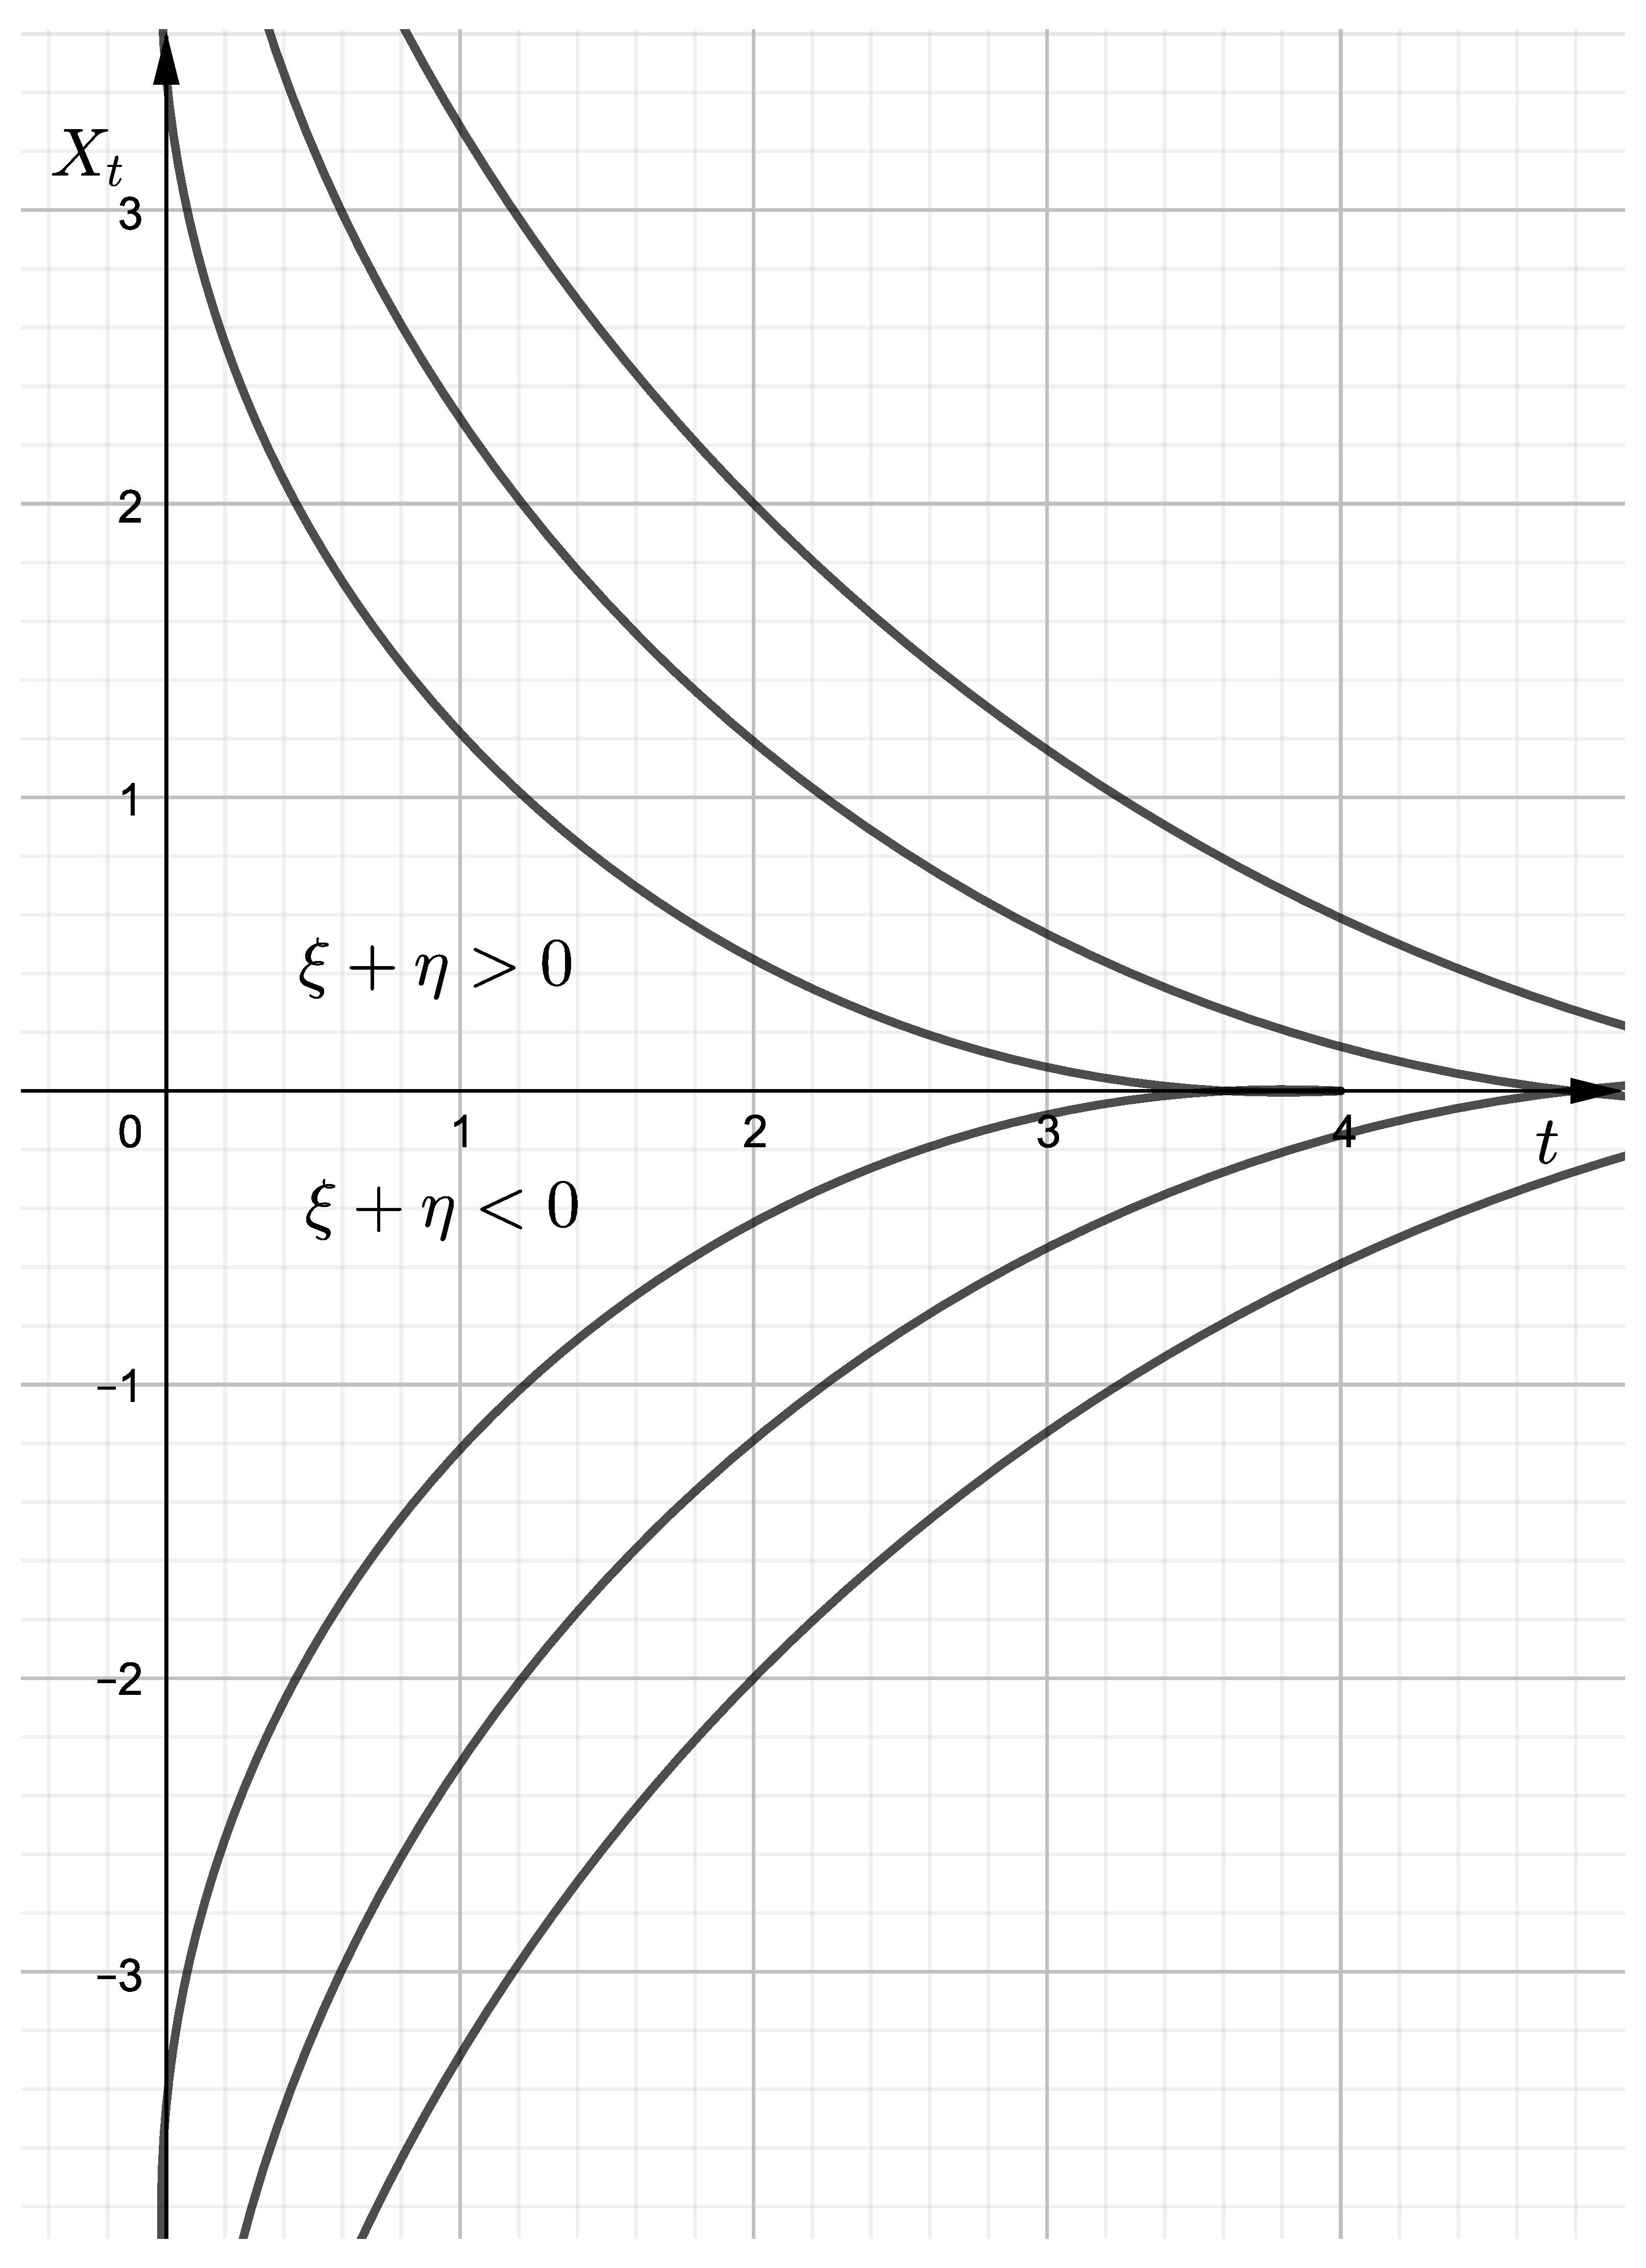
\includegraphics[width = 0.5\linewidth]{12}
	\caption{Траектории}
	\label{traj}
\end{figure}	


\subsubsection{i}
Случайный процесс описан уравнением $ X_{t}=e^{\xi t} $

В зависимости от того, будет реализация случайной величины положительной или отрицательной, кривые будут либо экспоненциально возрастать, либо экспоненциально убывать, где $ \xi $ будет служить коэффициентом скорости роста. Чем ближе $ \xi $ к единице, тем быстрее будет возрастать кривая траектории, а чем ближе к минус единице, тем быстрее убывать. Соответственно, семейство кривых ограничено сверху кривой $ X_t = e^\xi $, а снизу -- кривой   $ X_t = e^{-\xi} $. Графики возможных траекторий можно увидеть на Рис. \ref{traj} слева.

Найдём конечномерные распределения процесса. Для простоты записи покажу на двумерном примере, а далее разширим до многомерного случая.

\begin{enumerate}[\Sun]
	\item Очевидно, что $ P\{X_1 \le x_1, X_2 \le x_2\} = 0 $ при $ x_1 \le 0 или х_2 \le $, так как показательнаяя функция от экспоненты не может быть отрицательной или нулевой.
	
	\item При $ x_1 \ge 1 \text{ и } x_2 \ge 1 $ :

	\begin{equation}
	\begin{aligned}
	 P\{X_1 \le x_1, X_2 \le x_2\}=  P\{e^{\xi t_1}& \le x_1, e^{\xi t_2} \le x_2\} = P\{\xi t_1 \le ln(x_1), \xi t_2 \le ln(x_2)\} =\\ P\{ \xi \le min\left(\frac{ln(x_1)}{t_1}, \frac{ln(x_2)}{t_2}\right) \} 
	 \end{aligned}
	 \end{equation}
	 
	 \item При $ x_1 \ge 1 \text{ и } 0 < x_2 < 1 $ :
	 
 	\begin{equation}
 	\begin{aligned}
	 P\{X_1 \le x_1, X_2 \le x_2\}=  P\{e^{\xi t_1}& \le x_1, e^{\xi t_2} \le x_2\} = P\{\xi t_1 \le ln(x_1), \xi t_2 \le ln(x_2)\} = \\  P\{ \xi \le min\left(\frac{ln(x_1)}{t_1}, \frac{ln(x_2)}{t_2}\right) \} 
	 \end{aligned}
	 \end{equation}
	 
	 Так как $ ln(x_2) $ , будет отрицательным, $ ln(x_1) $ - положительным, то $  P\{ \xi \le \frac{ln(x_2)}{t_2} \} $ будет ответом в данном случае. 
	 
	 \item При $ x_2 \ge 1 \text{ и } 0 < x_1 < 1 $ :
	 
	 Абсолютно аналогично предыдущему случаю
	 
	 \item При $ 0 < x_2 < 1 \text{ и } 0 < x_1 < 1 $ :
	 
	$  P\{X_1 \le x_1, X_2 \le x_2\}= \cdots  P\{ \xi \le min\left(\frac{ln(x_1)}{t_1}, \frac{ln(x_2)}{t_2}\right) \}  $
	
	В данном случае оба числа будут отрицательными и формула останется без сокращений.
	
	Очевидно (нет, ну правда очевидно, можно я не буду объяснять?), что в многомерном случае будет ровно то же самое. Следовательно, без потери общности, можно записать ответ в сокращённом виде:
	
	$ F_\xi(x_1, \cdots, x_n) = P\{X_1 \le x_1,\cdots, X_n \le x_n\} = 
	\begin{cases}
		0, \text{ если }  \exists j \text{ s.t. } x_j <= 0, j = 1:n \\
		F_\xi\left(min\left(\frac{ln(x_1)}{t_1},  \cdots, \frac{ln(x_n)}{t_n}\right) \right)
	\end{cases} $
	
	где $ F_\xi(x) $ - функция распределения равномерной случайной величины $ \xi $ на $ [-1, 1] $
	 
\end{enumerate}

\subsubsection{ii}
Случайный процесс описан уравнением $X_{t}=(\xi+\eta) / t$. В зависимости от того, будет ли реализация случайной величины $ \xi + \eta $ положительной или отрицательной, траекториями будут семейства гипербол. Соответственно, чем ближе к нулю будет реализована данная случайная величина, тем более вогнуты будут гиперболы вогнуты в сторону точки (0.0). Графики возможных траекторий можно увидеть на Рис. \ref{traj} справа.


Что же касается конечномерного распределения, то здесь всё довольно похоже на предыдущий пунктб поэтому напишу с минимумом подробностей. Решим для двумерного случая и расширим на многомерный.

 Для начала, однако, установим параметры нормального распределения случайной величины $ \xi + \eta $. Математическое ожидание ноль. Ковариация двух величин тоже ноль, так что дисперсия равна 1. Получим стандартную нормальную величину.

\[  P\{X_1 \le x_1, X_2 \le x_2\} = P\{ \xi + \eta \le x_1 t_1, \xi + \eta \le x_2 t_2 \} = P\{ \xi + \eta \le min(x_1 t_1, x_2 t_2) \} \]

Рассмотрим 4 случая:

\begin{enumerate}[\Sun]
	\item $ x_1 \le 0, x_2 \le 0 $
	
	В данном случае обе величины $ x_1 t_1, x_2 t_2 $ будут отрицательными и ответ будет: $ F_{N_{(0,1)}}(min(x_1 t_1, x_2 t_2)) $
	
	\item $ x_1 \ge 0, x_2 \ge 0 $ 
	Очевидно, обе величины $ x_1 t_1, x_2 t_2 $ будут положительными и ответ:$ F_{N_{(0,1)}}(min(x_1 t_1, x_2 t_2)) $
	
	\item $ x_1 > 0, x_2 < 0 $ 
	
	$ x_1 t_1 $ будет положительной величиной, а $ x_2 t_2 $ - отрицательной. Ответ: $ F_{N_{(0,1)}}(min(x_1 t_1, x_2 t_2)) = F_{N_{(0,1)}}(x_2 t_2) $
	
	\item $ x_1 < 0, x_2 > 0 $ 
		Ответ зеркален предыдущему. 
		
\end{enumerate}
Очевидно, что с повышением размерности ни один из этих вариантов не будет нарушаться. При наличии хотя бы одной отрицательной переменной $ x_j $ среди положительных, она автоматически станет минимумом, а при всех переменных одного знака формула и вовсе не упрощается. Следовательно, без потери общности, запишем ответ:

\[  	 F_\xi(x_1, \cdots, x_n) = P\{X_1 \le x_1,\cdots, X_n \le x_n\} =  F_{N_{(0,1)}}(min(x_1 t_1, \cdots, x_n t_n)) \]

\subsection{Задача 2}

\[ P\{X_{t_1} < X_{t_2}\} = P\{t_1(\xi_1 + \alpha(\xi_2 + 2\alpha))<t_1(\xi_1 + \alpha(\xi_2 + 2\alpha)) \}=  \]
\[
P\{ (t_1 - t_2)\xi_1 + (t_1 - t_2)\alpha \xi_2 < (t_2 - t_1)2\alpha^2\} = \\P\{ \xi_1 + \alpha\xi_2 \ge -2\alpha^2\} = P\{ \xi_1 + \alpha\xi_2 + 2\alpha^2 \ge 0\} = 1\]
	
	
Чтобы вероятность того, что эта случайная величина была положительной стала равной единице, рассмотрим график. Так как указано, что параметр $ \alpha $ является реальным числом, будем рассматривать только случаи с положительным дискриминантом. Чтобы учесть максимальное количество случаев, при которых значение функции в точке положительно, максимально "опустим" параболу, максимизировав дискриминант. Очевидно, что это произойдёт в двух точках относительно $ \xi $: (1, -1), (-1, -1)

\[ D = \xi_2^2 - 8\xi_1 \]

\[ \alpha_1 = \frac{-\xi_2 - \sqrt{\xi_2^2 - 8\xi_1}}{4} \]

\[ \alpha_1 = \frac{-\xi_2 + \sqrt{\xi_2^2 - 8\xi_1}}{4} \]


Все мозможные случаи корней при $ \xi_2 = +- 1 $:
\[ 
\begin{cases}
	\alpha_{11} = -\frac{1}{2}\\
	\alpha_{12} = -1\\
	\alpha_{21} = \frac{1}{2}\\
	\alpha_{22} = 1
\end{cases}
 \]

Следовательно, при $ \alpha \in [-1, 1] $ все возможные параболы будут принимать только неотрицательные значения.
Ответ:  $ \alpha \in [-1, 1] $ 

\subsection{Задача 3}

\[  f _ { z } ( x ) = \frac { 1 } { 2 } e ^ { - x } + e ^ { - 2 x } , x > 0  \]

\begin{equation}
\begin{aligned}  L [ p ] ( u ) = \int _ { 0 } ^ { \infty } \left( \frac { 1 } { 2 } e ^ { - x } + e ^ { - 2 x } \right) e ^ { - u x } d x  = \int _ { 0 } ^ { \infty } \frac { 1 } { 2 } e ^ { - x ( 1 + u ) } + e ^ { - x ( 2 + u ) } d x = \\ = \frac { 1 } { 2 ( 1 + u ) } + \frac { 1 } { 2 + u } = \frac { 2 + u + 2 + 2 u } { 4 + 4 u + 2 u + 2 u ^ { 2 } } =  \frac { 4 + 3 u } { 2 u ^ { 2 } + 6 u + 4 } \end{aligned}
\end{equation}

\begin{equation}
\begin{aligned}
L [ U ] ( u ) = \frac { \frac { 4 + 3 u } { 2 u ^ { 2 } + 6 u + 4 } } { u \left( 1 - \frac { 4 + 3 u } { 2 u ^ { 2 } + 6 u + 4 } \right) } = \frac { \frac { 4 + 3 u } { 2 u ^ { 2 } + 6 u + 4 } } { u \left( \frac { 2 u ^ { 2 } + 3 u } { 2 u ^ { 2 } + 6 u + 4 } \right) }= \frac { 3 u + 4 } { 2 u ^ { 3 } + 3 u ^ { 2 } } = \frac { 3 u  + 4 } { u ^ { 2 } ( 2 u + 3 ) } 
\end{aligned}
\end{equation}




\[ 
\frac { 3 u + 4 } { u ^ { 2 } ( 2 u + 3 ) } = \frac { A } { u } + \frac { B } { u ^ { 2 } } + \frac { C } { u + 3 }  = \frac { A u ( 2 u + 3 ) + B ( 2 u + 3 ) + C u ^ { 2 } } { u ^ { 2 } ( 2 u + 3 ) } = \frac { 2 A u ^ { 2 } + C u ^ { 2 } + 3 A u + 2 B u + 3 B } { u ^ { 2 } ( 2 u + 3 ) }
 \]

\begin{equation}
\left\{ \begin{array} { l } { C + 2 A = 0 } \\ { 3 A + 2 B = 3 } \\ { 3 B = 4 } \end{array} \Rightarrow \left\{ \begin{array} { l } { A = \frac { 1 } { 9 } } \\ { B = \frac { 4 } { 3 } } \\ { C = - \frac { 2 } { 9 } } \end{array} \right. \right.
\end{equation}


\[ U(t) = \frac{1}{9} + \frac{4}{3}t - \frac{1}{9}\exp^{-\frac{3}{2}t}\]

\subsection{Задача 4}
\subsubsection{i}

 \begin{wrapfigure}{l}{0.4\textwidth}
	\includegraphics[width=\linewidth]{13}
	\caption{$  f_{\xi - \eta}(x) $}
	\label{minmax}
\end{wrapfigure}


Для начала выведем несколько необходимых свойств функций плотностей.
\begin{equation}
\begin{aligned}
	F_{|\xi|} = P\{|\xi| \le x\}  = P\{-x \le \xi \le x \} =\\ P\{\xi \le x \} - P\{\xi \le -x \} = F_\xi(x) - F_\xi(-x) 
\end{aligned}
\end{equation}
Следовательно:
 \[ f_{|\xi|}(x) = f_\xi(x) + f_\xi(-x) \] 
 
 Теперь по формуле свёртки выведем следующую плотность:
 
 \[ f_{\xi - \eta}(x) = f_{\xi + (-\eta)}(x) \]
 
Для этого выведем следующее свойство:

 
\[  F_{-\eta}(x) = P\{-\eta \le x\} = P\{\eta \ge -x\} =\\ 1 -F_{\eta}(-x) \Rightarrow f_{-\eta}(x) = f_{\eta}(-x) \] 

Теперь возьмём интеграл:


\[  f_{\xi - \eta}(x) = \int_{-\infty}^{\infty} I\{u - x \in [0;1]\} I\{- x \in [0;1]\} = \int_{max(u-1,-1)}^{min(u,0)}1 dx = min(u,0) - max(u-1,-1) \]

Полученная фукнция изображена на \ref{minmax}.

Так как функция симметричная, $ f_{|\xi|}(x) = f_\xi(x) + f_\xi(-x) = 2 f_\xi(x) $. Следовательно: 

\[  f_{|\xi - \eta|}(x) = 2(min(u,0) - max(u-1,-1))  \]

Однако следует сделать важное замечание. Так как модуль случайной величины неотрицателен, складывать функции распределения следует только на положительной полуоси. Таким образом, ответ:

\[  f_{|\xi - \eta|}(x) = 
\begin{cases}
0, u < 0\\
2(min(u,0) - max(u-1,-1)), u \ge 0
\end{cases}
 \]
 
 Нетрудно проверить, что эта функция будет соответствовать всем необходимым свойствам функции плотности.


\subsubsection{ii}

По формуле свёртки:
\begin{equation*}
\begin{aligned}
f_{\xi + \eta} = \int_{-\infty}^{\infty} \frac{1}{4} \exp^{-|u-x|-|x|} dx=  \frac{1}{4}  \left( \int_{-\infty}^{0} \exp^{-|u-x|+x} dx + \int_{0}^{\infty}  \exp^{-|u-x|-x} dx \right) = \\ \frac{1}{4} \left( \int_{-\infty}^{min(u,0)} \exp^{-u+2x} dx+ \int_{min(u,0)}^{0} \exp^{u} dx+ \int_{0}^{max(u,0)}  \exp^{-u} dx + \int_{max(u,0)}^{+\infty}  \exp^{u-2x} dx \right) = \\
\frac{1}{4} \left( \frac{1}{2}\exp^{-u+2x} \Biggr|_{-\infty}^{min(u,0)}  + x \exp^u \Biggr|_{min(u,0)}^{0} + x \exp^{-u} \Biggr|_{0}^{max(u, 0)}  - \frac{1}{2} \exp^{u-2x} \Biggr|_{max(u, 0)}^{+\infty} \right) = \\
\frac{1}{4} \left( \frac{1}{2}\exp^{-u+2min(u,0)} - min(u,0) \exp^u + max(u,0) \exp^{-u} + \frac{1}{2} \exp^{u-2max(u, 0)} \right)
\end{aligned}
\end{equation*}

Вольфрам сказал, что интеграл под этой функцией равен единице, так что всё должно быть верно. По форме распределение напоминает нормальное. Касательно возникших функций минимума и максимума, они призваны регулировать функцию в зависимости от знака параметра $ u $. В зависимости от него один из четырёх интегралов во 2 строке будет схлопываться в нулевой.

\subsection{Задача 5}

\subsubsection{i}

Нет, не является процессом восстановления, так как $ p\{ \xi_i \ge 0 \} \neq 1 $

\subsubsection{ii}
Каждая траектория имеед вид ломаной кривой. Она начинается в точке ноль и образует один из путей (слева направо) в древовидной структуре на Рис.  \ref{rombs}.Для примера одна из возможных траекторий окрашена в оранжевый. Данная фигура по виду очень напоминает треугольник Паскаля.


\begin{figure}[h]
	\includegraphics[width=0.3\linewidth]{14}
	\caption{Траектории $ S_n $}
	\label{rombs}
\end{figure}
\subsubsection{iii}

Сколько-нибудь адекватный ответ в явном виде у меня не получился, остался только следующий вариант:

\begin{equation*}
\begin{aligned}
P\{  X_1 \le x_1, X_2 \le x_2, \cdots, X_n \le x_n \}  = P\{  X_1 \le x_1, X_2 \le x_2, \cdots, X_n \le x_n \} =\\
P\{  \sum_{i = 1}^{t_1}\xi_i \le x_1, \sum_{i = 1}^{t_2}\xi_i \le x_2, \cdots, \sum_{i = 1}^{t_n}\xi_i \le x_n \} = \\ P\{  \sum_{i = 1}^{t_1}\xi_i \le x_1, \sum_{i = t_1 + 1}^{t_2}\xi_i \le x_2 - x_1, \cdots, \sum_{i = t_{n-1}+1}^{t_n}\xi_i \le x_n - x_{n-1} \}
\end{aligned}
\end{equation*}




Логика такого перехода в следующем:

\[ \sum_{t_1 + 1}^{t_2}\xi_i + x_1 \le \sum_{1}^{t_2} \xi_i \le x_2 \Rightarrow \sum_{t_1 + 1}^{t_2} \xi_i \le x_2 - x_1\]

Нетрудно проверить, что для каждого периода необходимо просто вычитать предыдущий. Я не доконца уверен в этом переходе, но выглядит красиво. Теперь события независимы. Можно разбить на произведение свёрток в смысле распределений:


\begin{equation*}
\begin{aligned}
 P\{  \sum_{i = 1}^{t_1}\xi_i \le x_1, \sum_{i = t_1 + 1}^{t_2}\xi_i \le x_2 - x_1, \cdots, \sum_{i = t_{n-1}}^{t_n}\xi_i \le x_n - x_{n-1}\} =&\\ F^{*t_1}(x_1) \cdot F^{*(t_2 - t_1)}(x_2 - x_1) \cdot \cdots \cdot F^{*(t_n - t_{n-1})}(x_n - x_{n-1})
\end{aligned}
\end{equation*}

Единственное ограничение, которое можно наложить на переменные, это что при  $ x_j - x_{j-1}  < t_j - t_{j-1}$ выражение $ \sum_{i = t_{j-1} + 1}^{t_j}\xi_i $ обратится в ноль. Это случится потому что сумма описанных выше величин не может быть мешьше чем (-1) * (количество величин в сумме). Итоговый ответ можно записать следующим образом:

$ F_\xi(x_1, \cdots, x_n) =
\begin{cases}
	0, \text{ если } \exists \text{ j s.t. } x_j - x_{j-1}  < t_j - t_{j-1} \\
 F^{*t_1}(x_1) \cdot F^{*(t_2 - t_1)}(x_2 - x_1) \cdot \cdots \cdot F^{*(t_n - t_{n-1})}(x_n - x_{n-1}) \text{ иначе }
\end{cases}
$

Мне самому не очень нравится этот ответ, так как она не даёт идей для следующего пункта и так как эти непонятные свёртки вообще неясно как брать в случае дискретных величин. 


\subsubsection{iv}

\subsection{Задача 6}

Данное утверждение неверно. (Иначе бы его дали в лекции как более общее, ну логично же)

Событие $ \{N_t \le n\}$ можно интерпретировать следующим образом. Возможны три варианта событий:

\begin{enumerate}[\Sun]
	\item	К моменту времени $ t $ появилось менее n клиентов. 
	
	\item В момент времени $ t $ подошёл $ n $-ый покупатель.
	
	\item В какой-то из моментов времени до $ t $ подошёл $ n $-ый покупатель, и вплоть до момента $ t $ более покупателей не приходило
\end{enumerate}

Следовательно:
\[  \{N_t \le n\} = \{S_n > t\} \cup \{S_n = t\} \cup \{S_n < t\} \neq \{S_n \ge t \} =  \{S_n > t\} \cup \{S_n = t\}  \]

Исходное утверждение неверно.


\section{Домашнее задание 2}

\subsection{Задача 1}

Начальное условие: $ Z_0 = c $

Обозначим случайную величину $ \tau $ следующим образом: 

\[\tau = \begin{cases}
1,  1-F_\eta(R)\\
0, F_\eta(R)
\end{cases}  \]

Пусть $ \E(\xi_n) = \mu $

Процесс восстановления: $ Z_n = Z_{n-1} + \tau_n \xi_n $

Вычтем начальное условие из обоих частей:

\[ Z_n - c = Z_{n-1} - c + \tau_n \xi_n \]

Переобозначим:

\[  S_n = S_{n-1} + \tau_n \xi_n  \]

$ N_t = max\{ k, S_k \le t \} = max\{ k, Z_k - c \le t \} = max\{ k, Z_k \le t + c\} = M(C) $

\[ t + c = C \Rightarrow t = C - c  \]

\[ \lim\limits_{t \to \infty} \frac{N_t}{t} = \frac{1}{\E(\tau \xi_n)} = \frac{1}{(1 - F_\eta(R))\mu} = \lim\limits_{C \to \infty} \frac{M(C)}{t(C)} \]

\[ \E(\tau \xi_n) = \text{ независимость } = (1 - F_\eta(R)) \mu \]


\[ \lim\limits_{C \to \infty} \frac{M(C)}{t(C)} =  \frac{1}{(1 - F_\eta(R))\mu} \Rightarrow  \lim\limits_{C \to \infty} M(C) = \frac{C - c}{(1 - F_\eta(R))\mu} \]

\subsection{Задача 2} 

\subsubsection{i}
 
 Это событие будет подчиняться геометрическому распределению. По всем известной формуле математического ожидания это будет $ \frac{1}{p} $

\subsubsection{ii}

Процесс восстановления: $ S_n = S_{n-1} + \xi_n $

$ \E \xi_i = 45 $

Обозначим индикатор обнаружения :

\[\tau = \begin{cases}
1,  p\\
0, 1-p
\end{cases}  \]

Штраф: $ \zeta \sim U[0, C(\frac{A}{B})],  $

Вознаграждение случайного процесса:  $ R_i = \tau \zeta  \Rightarrow \text{ независимость } \Rightarrow \E(R_i) = \frac{p C}{2}$

\[ \frac{Y(t)}{t} \to \frac{p C}{90} \Rightarrow Y(t) \to \frac{\tau p C}{90}\]


\subsubsection{iii}

Рассмотрим две альтернативы поведения. Первый вариант поведения владельца это экономия. Усредним возможные профиты и лоссы. В таком случае в любой конкретный день он в среднем будет получать профит $ A - B $. Константу сколько не усредняй, останется константой. Однако он будет в среднем получать асимптотическиий штраф  $ Y(t) \to \frac{\t p C}{90} $, который мы вычислили в предыдущем пункте.

В ином вариант, когда владелец выбирает не экономить, он не получает выгоды, но в среднем каждый день теряет $ А $ рублей.

 В таком случае владельцу будет выгодно экономить, если средяя "чистая прибыль" от экономии будет больше, чем от экономии, то есть:
 
 \[ A - B - \frac{Y(t)}{t} > -A \]
 
 \[ A - B - \frac{p C}{90} > -A \]
 
 В таком случае владельцу будет выгодна первая стратегия даже если чистая прибыль от экономии будет отрицательной из-за штрафов, но будет больше чем $ -A $, то экономия всё равно останется оптимальной. Преобразуя неравенство, получим:
 
 \[  2A - B - \frac{pC}{90} > 0 \Rightarrow \frac{90(2A-B)}{C(\frac{A}{B})} > p\]
 
 Если честно, я не понял, как использовать зависимость $ С $ от дроби. Разве что наложить дополнительные условия на производную $ C $ по $ A $ и $ B $. Возможно это даст какие-то дополнительные условия на $ C $, но особого смысла в этом не вижу.
 
 \subsection{Задача 3}
 
 Выпишем суммарное вознаграждение процесса востановления. Для начала обозначим пару вспомогательных индикаторов. $ \tau $ -- индикатор того, что ремонт возможно произвести самостоятельно. $ \rho $ -- индикатор того, что самостоятельный ремонт был некачественным. \
 
 \[\tau = \begin{cases}
 1,  p\\
 0, 1-p
 \end{cases}  \]
 
  \[\rho = \begin{cases}
 1,  q\\
 0, 1-q
 \end{cases}  \]
 
 \[ R_i = \tau \rho (m + \eta) + \tau (1-\rho)m + (1 - \tau) \eta \]
 

\subsubsection{i}

В данном пункте необходимо только первое слагаемое. При $  t \to \infty $ уммарные расходы будут следующими:

\[ \frac{Y(t)}{t} \to \frac{\E(R_i^I)}{\E(\xi_i)} = \text{независимость} = \frac{pq\left(m + \frac{M + m}{2}\right)}{18} \Rightarrow Y(t) \to \frac{tpq\left(m + \frac{M + m}{2}\right)}{18}  \]

\subsubsection{ii}

Сравним ожидаемые вознаграждения за самостоятельный ремонт и за ремонт в автосервисе. Первое должно быть меньше второго. По-хорошему, нужно обе части неравенства ниже делить на $ \E(xi_i) $б но все понимают, что я просто мысленно на это же положительное число 18 просто домножил обе части чтобы лишние дроби не тянуть. Матожидания позволю себе также вычислить в уме.

\begin{equation}
\begin{aligned}
pq\left(m + \frac{M + m}{2}\right) + p(1-q)m < \frac{(1-p)(M+m)}{2} \Rightarrow \Big| *2 \text{ и } :q\\
q(M + 3m) + 2m(1-q) < \frac{M+m}{p} - (M + m) \Rightarrow \Big| :(M+m) \\
\frac{q(M + 3m) + 2m - 2qm}{M+m} < \frac{1 - p}{p} \Rightarrow
\frac{qM + qm + 2m}{M + m} < \frac{1 - p}{p} \Rightarrow \\
q + \frac{2m}{M + m} < \frac{1 - p}{p} 
\end{aligned}
\end{equation}

\subsection{Задача 4}

\begin{figure}[h]
	
	\includegraphics[width = 0.5\linewidth]{21}
	\includegraphics[width = 0.5\linewidth]{22}
	\label{police}
\end{figure}

Как и в лекции, будем пользоваться теоремой о двух милиционерах. Это до ужаса скучно, но так и быть. Поправка к графикам, которые у меня уже нет сил перерисовывать: по оси ординат, конечно же, $ \xi_1, \xi_2 ... $? а не $ S_1, S_2 ... $

\subsubsection{i}

Функция под интегралом представляет собой просто куски прямой $ Z(t) = t $, которя в каждый момент восстановления просто сдвигается на $ \xi_i $.
Как видно из графика слева на Рис. \ref{police}, искомый интеграл ограничен суммами площадей треугольников до точек $ N_t $ и $ N_t+1 $. Найдём пределы границ неравенства.

\[ \frac{\sum_{1}^{N_t}\frac{1}{2}\xi_i^2}{t} \le \int_{0}^{t}Z_u^{w} du\le \frac{\sum_{1}^{N_t + 1}\frac{1}{2}\xi_i^2}{t} \]

\[ \lim\limits_{t \to \infty}\frac{1}{2t} \sum_{1}^{N_t}\xi_i^2 = \lim\limits_{t \to \infty} \frac{N_t}{t}  \frac{\sum_{1}^{N_t}\xi_i^2 }{2 N_t} = \frac{\E(\xi_1^2)}{2 \E(\xi_1)} \]


\[ \lim\limits_{t \to \infty}\frac{1}{2t} \sum_{1}^{N_t + 1}\xi_i^2 = \lim\limits_{t \to \infty}\frac{1}{2t} \sum_{1}^{N_t + 1}\xi_i^2 \frac{N_t + 1}{N_t}  \frac{N_t}{N_t+1}= 
\lim\limits_{t \to \infty} \frac{N_t}{t}  \frac{\sum_{1}^{N_t}\xi_i^2 }{2 N_t} \frac{N_t + 1}{N_t} = \frac{\E(\xi_1^2)}{2 \E(\xi_1)} \]

Видим, что исходная функция зажата двумя абсолютно идентичными функциями. Следовательно, по теореме о двух милиционерах предел исходной функции тоже будет равен $ \frac{\E(\xi_1^2)}{2 \E(\xi_1)} $




\subsubsection{ii}

Пункт абсолютно идентичен предыдущему. Единственная разница лишь в построении графика. Искомое время является ни чем иным как $ \xi_{N_t+1} $. Скачки графика происходят непосредственно в моменты восстановления. Все вычисления и выводы абсолютно идентичны, с поправкой на $ \frac{1}{2} $, так как площадь каждого квадрата будет ровно $ \xi_i^2 $.


\[ \frac{\sum_{1}^{N_t}\xi_i^2}{t} \le \int_{0}^{t}V_u^{w} du\le \frac{\sum_{1}^{N_t + 1}\xi_i^2}{t} \]

\[ \lim\limits_{t \to \infty} \sum_{1}^{N_t}\xi_i^2 = \lim\limits_{t \to \infty} \frac{N_t}{t}  \frac{\sum_{1}^{N_t}\xi_i^2 }{N_t} = \frac{\E(\xi_1^2)}{\E(\xi_1)} \]

\[ \lim\limits_{t \to \infty} \sum_{1}^{N_t + 1}\xi_i^2 = \lim\limits_{t \to \infty} \sum_{1}^{N_t + 1}\xi_i^2 \frac{N_t + 1}{N_t}  \frac{N_t}{N_t+1}= 
\lim\limits_{t \to \infty} \frac{N_t}{t}  \frac{\sum_{1}^{N_t}\xi_i^2 }{ N_t} \frac{N_t + 1}{N_t} = \frac{\E(\xi_1^2)}{ \E(\xi_1)} \]

Видим, что исходная функция зажата двумя абсолютно идентичными функциями. Следовательно, по теореме о двух милиционерах предел исходной функции тоже будет равен $ \frac{\E(\xi_1^2)}{ \E(\xi_1)} $


\subsection{Задача 5}

\subsection{Задача 6}

\subsubsection{i}

\[  \E(S_{N_t+1}) = \mu \E(N_t) + \mu\]

Далее сделаем ключевой переход. $ S_{N_t+1} $ это точка времени, в которую произойдёт следующий после точки $ t $  эпизод восстановления. Очевидно, что математическое ожидание этой случайной величины больше $ t $, так как это событие должно произойти после $ t $. Следовательно:

\[  \E(S_{N_t+1}) = \mu \E(N_t) + \mu > t \Rightarrow \E(N_t) > \frac{t}{\mu} - 1 \Rightarrow \frac{\E(N_t)}{t} > \frac{1}{\mu} - \frac{1}{t}\]

\subsubsection{ii}

Снова воспользуемся тождеством Вальда. Начём доказывать с конца.

\[ \E(\tilde{N}_t)  \le \frac{t}{\tilde{\mu}(\sqrt{t})} + \frac{\sqrt{t}}{\tilde{\mu}(\sqrt{t})} \Rightarrow  \tilde{\mu}(\sqrt{t}) \E(\tilde{N}_t) \le t + \sqrt{t} \]

Согласно тождеству Вальда:

\[ \E(S_{N_t}) =  \tilde{\mu}(\sqrt{t}) \E(\tilde{N}_t) \]


Следовательно:
\[  \E(S_{N_t}) \le t + \sqrt{t}  \]

Данное неравенство выполняется всегда, так как событие $ S_{N_t} $ -- последний момент восстановлления до $ t $, и его математическое ожидание должно быть меньше $ t $. Следовательно, получаем тождество. Исходное предположение доказано.

Что же касается левой части неравенства, её можно доказать интуитивно. Так как в процессе восстановления в приращениях всегда будет прибавляться меньший чем $ \xi_n $ отрезок времени $ \tilde{\xi}_n $, то до момента времени $ t $ произойдёт точно не меньше эпизодов восстановлени (если все реализации случайной величины $ \xi_n $ будут больше $ b $) или больше. Следовательно, математическое ожидание количества восстановлений к моменту $ t $ тоже будет выше. 

Оба положения неравенства доказаны.

\subsubsection{iii}

После первых двух пунктов получаем неравенство:

\[ \frac{1}{\mu} - \frac{1 }{t}  < \frac{\E(N_t)}{t} < \frac{1}{\tilde{\mu}(\sqrt{t})} +\frac{1}{\sqrt{t}\tilde{\mu}(\sqrt{t})} \]

Теперь, очевидно, как и в задаче 4, нужно воспользоваться теоремой о двух милиционерах. Но сначала нужно доказать, что $\tilde{\mu}(\sqrt{t}) \rightarrow \mu \operatorname{ при } t \rightarrow \infty$

Для этого нужно вычислить следующее:

\[  \lim\limits_{t \rightarrow +\infty}   \E(min(\sqrt{t}, \xi_n)) \]

Для этого так и напрашивается поменять местами предел и математическое ожидание. Однако для этого нужно выполнить условия Dominated convergence theorem. Как бы по-хорошему нужно выписать все предпосылки о вероятностном пространстве как метрическом пространстве и обозначить предпосылки, но сил уже на это мало. Обозначим самые главные. Нужно найти такую мажорирующую функцию $ g $, что:

\begin{enumerate}[\Sun]
	\item Функция плотности $ g $ должна быть интегрируема
	
	\item Математическое ожидание модуля $ g $ конечно
	
	\item Функция $ g  $ должна доминировать исходную функцию.
\end{enumerate}

Всё просто. Обозначим $ g = \xi_n $. Её математическое ожидание конечно по условию, и мы можем менять в исходном неравенстве предел и математическое ожидание.

Можно проиллюстрировать всё следующим примером.

Очевидно, что:
\[ min(b, \xi_n) \le \xi_n\]

Это было как раз условие доминирования. Оно верно с учётом того, что $  \xi_n $ неотрицательная случайная величина. Домножим на неотрицательную функцию плотности.

\[f_\xi(x) min(b, \xi_n) \le f_\xi(x)\xi_n \]

Возьмём математическое ожидание обеих частей:

\[ \int_{0}^{+\infty} f_\xi(x) min(\sqrt{t}, x) dx \le \int_{0}^{+\infty} f_\xi(x) x dx \]


Математическое ожидание исходной функции тоже доминировано конечным математическим ожиданием $ \xi $

По пунктам. Нужно ввести предпосылку о том, что функция плотности $ \xi $ интегрируема. Математическое ожидание модуля $ \xi $ равно математическому ожиданию $ \xi $ и конечно. Очевидно, что $ \xi_n $  доминирует исходную функцию.

Поменяем предел и математическое ожидание:

\[  \lim\limits_{t \rightarrow +\infty}   \E(min(\sqrt{t}, \xi_n)) \Rightarrow    \E( \lim\limits_{t \rightarrow +\infty}  min(\sqrt{t}, \xi_n)) = \E(\xi_n)  = \mu\]


Следовательно, мы доказали, что $\tilde{\mu}(\sqrt{t}) \rightarrow \mu \operatorname{ при } t \rightarrow \infty$. Теперь воспользуемся-таки теоремой о двух милиционерах и возьмём пределы по двум границам исходного неравенства:


\[ \frac{1}{\mu} - \frac{1 }{t}  < \frac{\E(N_t)}{t} \le \frac{1}{\tilde{\mu}(\sqrt{t})} +\frac{1}{\sqrt{t}\tilde{\mu}(\sqrt{t})} \]

Очевидно, что при $ t \to +\infty $ дроби с $ t $ в знаменателях занулятся, а в правой части по доказанной выше сходимости появится тоже $ \nu $ В итоге:

\[ \frac{1}{\mu}   <  \lim\limits_{t \rightarrow +\infty} \frac{\E(N_t)}{t} \le \frac{1}{\mu}  \]

Следовательно, получаем: 

\[  \lim\limits_{t \rightarrow +\infty} \frac{\E(N_t)}{t} = \frac{1}{\mu}    \]




\end{document}
